\documentclass{UTNetLab}
\usepackage[bottom]{footmisc}


\title{The Web, DHCP, NTP and NAT}
\newcommand\reference{
   S. Panwar, S. Mao, J.-dong Ryoo, and Y. Li, “The Web, DHCP, NTP and NAT,” in TCP/IP Essentials: A Lab-Based Approach, Cambridge: Cambridge University Press, 2004, pp. 159–186.
}

\begin{document}
	\section*{Objectives}
	\begin{itemize}
		\item The HyperText Transfer Protocol (HTTP) and the Apache web server.
		\item The Common Gateway Interface (CGI) and other web-server app (like PHP, Ruby, Python, \dots).
		\item The Dynamic Host Configuration Protocol (DHCP).
		\item The Network Time Protocol (NTP).
		\item The Network Address Translator (NAT) and the Port Address Translator (PAT).
		\item [-] An introduction to socket programming.
	\end{itemize}
\part{HTTP Exercises}
For the exercises in this section, the network topology is simple with two hosts are connected to a single network segment with IP addresses, i.e.\  from 128.238.66.100 to 128.238.66.101.
You can use {Figure~3.server.gui}.
    
    \begin{figure}[H]
    	\centering
    	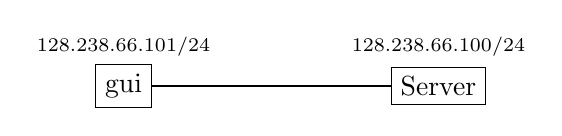
\begin{tikzpicture}
    	\node[draw] (Server) at (2,0){Server};
    	\node[draw] (gui) at (-2,0){gui};
    	
    	\draw (gui) -- (Server);
    	\draw (Server) +(0,0.5) node {\scriptsize 128.238.66.100/24};
    	\draw (gui) +(0,0.5) node {\scriptsize 128.238.66.101/24};
    
    	\end{tikzpicture}
    	\caption{One gui and one terminal host (Server) connected directly. (Figure~3.server.gui)}
    	\label{fig:two-gui}
    \end{figure}

\section{HTTP Server}
   Examine the various configuration directives used and the corresponding settings\footnote{\path{/etc/apache2/apache2.conf}}.
   
   Start the Apache server on  \textit{Server} by executing: 
       
	\fcolorbox{blue}{red!10}{{Server}'s Console}
	\lstset{backgroundcolor=\color{red!10}}
	\begin{lstlisting}
	service apache2 start
	\end{lstlisting}

    Double-click on the \textit{gui} client to bring it up. Then, from the start menu of the GUI, open \textit{Mozilla Firefox} (from the \textit{Internet} sub-menu) and enter the \textit{Server}'s IP address in the URL box:
    
    \fcolorbox{blue}{green!10}{\textit{gui}'s web browser}
    \lstset{backgroundcolor=\color{green!10}}
    \begin{lstlisting}
    http://128.238.66.100/
    \end{lstlisting}

    Then, execute the following command in \textit{Server} to list the process IDs of the \lstinline{apache2} processes started:
    
   	\fcolorbox{blue}{red!10}{{{Server}'s Console}}
    \lstset{backgroundcolor=\color{red!10}}
    \begin{lstlisting}
	pgrep apache2
    \end{lstlisting}
    
    Open the Multi-Processing Module config file with a text editor and study its various configurations and their applications by executing: 
    
    \fcolorbox{blue}{red!10}{{Server}'s Console}
    \lstset{backgroundcolor=\color{red!10}}
    \begin{lstlisting}
    nano /etc/apache2/mods-available/mpm_prefork.conf
    \end{lstlisting}
    
    Save the output and the configuration file for the lab report.
    
    \begin{report}
    \item How many \lstinline{apache2} processes were started?
    Which one was the master server, and which ones were the child servers? Use \lstinline{htop} in the \textbf{tree} mode to see process hierarchy by executing:
    
    \fcolorbox{blue}{red!10}{{Server}'s Console}
    \lstset{backgroundcolor=\color{red!10}}
    \begin{lstlisting}[xleftmargin=0.05in]
	htop --tree
    \end{lstlisting}
    
    Justify your answer using the \lstinline{apache2} configurations file. Explain your answer with values of \textit{Startservers, MinSpareServers, MaxSpareServers, MaxRequestWorkers, ServerLimit, MaxconnectionsPerChild}
    
    \item What is the purpose of initiating multiple \lstinline{apache2} processes? 
    \end{report}

\section{HTTP Request}
Execute \lstinline{wireshark} to capture packets between the \textit{gui} host and the \textit{server} host.

Login to the \textit{server} host’s web server by executing the following command in the \textit{gui}'s terminal: 

\textbf{Note: } To open the \textit{gui}'s terminal, from the start menu, choose \textit{System Tools} and then open \textit{LXTerminal}:

\begin{figure}[H]
	\centering
       {\selectlanguage{english}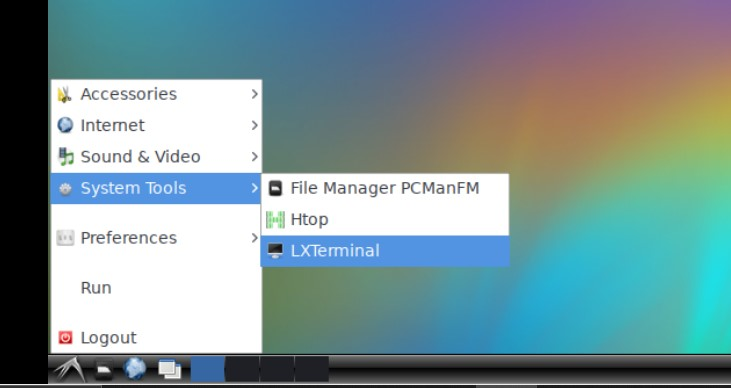
\includegraphics[scale=0.7]{img/gui.jpg}}
	\label{}
    \end{figure}
    
   	\fcolorbox{blue}{red!10}{{gui's Terminal}}
    \lstset{backgroundcolor=\color{red!10}}
    \begin{lstlisting}[emph={your-host, remote-host}]
    telnet 128.238.66.100 80
    \end{lstlisting}
    
    In the telnet console, type the following HTTP request line by line (type it fast enough before the connection gets closed, or simply copy-paste it):
    
   	\fcolorbox{blue}{red!10}{{gui's Terminal}}
    \lstset{backgroundcolor=\color{red!10}}
    \begin{lstlisting}[language={HTTP},escapechar={},emph={your-host, remote-host}]
	 GET /index.html HTTP/1.0
	 From: netlab@h0
	 User-Agent: HTTPTool/1.0
    \end{lstlisting}
    
    Note that you need to press the \textit{Return} key to input the last line, which is blank (you should press the \textit{Enter} key twice).
    When the \lstinline{telnet} process is terminated, save the output for your lab report. 

    Terminate \lstinline{wireshark} and analyze the captured HTTP packets.
    Print and save the HTTP request and response. 

    Save the HTTP response’s data part into a file, named \path{index.html}.
    Use \textit{Mozilla} to view the file.
    
    \begin{report}
    \item Submit the HTTP request and response, including the start-lines and all the headers.
    \end{report}

    
\section{HTTP \texttt{Keep-Alive}}
    By default, \textit{Apache} server supports persistent connections. Before this exercise, check the \texttt{KeepAlive} directive in the server configuration file to make sure that it is turned on as \lstinline[language={HTTP}]{KeepAlive On}. To do this, execute the following command and search for \lstinline{KeepAlive}:
	
    \fcolorbox{blue}{red!10}{{Server}'s Console}
    \lstset{backgroundcolor=\color{red!10}}
    \begin{lstlisting}
    nano /etc/apache2/apache2.conf
    \end{lstlisting}

    Run \lstinline{wireshark} to capture packets between the \textit{gui} host and the \textit{server} host.
    
    \fcolorbox{blue}{lime!30}{{gui}'s Wireshark}
    \lstset{backgroundcolor=\color{lime!30}}
    \begin{lstlisting}
    Run wireshark on eth1, Filter: ip.addr == 128.238.66.100 && ip.addr == 128.238.66.101
       
    \end{lstlisting}


    Enter the following URL in the \textit{gui}'s web browser to download the HTML file consisting a line of text, an embedded picture, and a hyperlink:
    
 	\fcolorbox{blue}{green!10}{gui's web browser}
	\lstset{backgroundcolor=\color{green!10}}
	\begin{lstlisting}
	http://128.238.66.100/try1.html
	\end{lstlisting}
	
    In \textit{Server}, disable the \textit{Apache} server persistent connections by changing the value of \texttt{KeepAlive} option to \lstinline{Off} from the configuration file (as mentioned above). To save the file after modifying it, press \lstinline{Ctrl+X}, confirm it by entering \lstinline{Y} and press enter. Then restart \lstinline{apache2} service by running following command:
    
    \fcolorbox{blue}{red!10}{{Server}'s Console}
    \lstset{backgroundcolor=\color{red!10}}
    \begin{lstlisting}
    service apache2 restart
    \end{lstlisting}
    
    Run \lstinline{wireshark} and print the HTTP requests and responses for the lab report.
    
    Use \textit{Mozilla} in  \textit{gui}'s to reload the \url{try1.html} file. Use \textit{Ctrl+F5} to ignore cache.

Use \lstinline{wireshark} and print the HTTP requests and responses for the lab report.

    \begin{report}
        \item When you browsed the \path{try1.html} file for the first time, how many HTTP requests were sent?
        Which files were requested?
        How many TCP connections were used?
        
        \item Answer the above questions for when you browsed the \path{try1.html} file for the second time.
        
        \item What is the purpose of using persistent connections?
    \end{report}



\section{HTTP Submit}
Execute \lstinline{wireshark} to capture packets between the \textit{gui} host and the \textit{server} host.

    Use \textit{Mozilla} in the  (\textit{gui}) to download the following file, which is an \textit{HTML} form, from the server.
     
    \fcolorbox{blue}{green!10}{\textit{gui}'s web browser}
	\lstset{backgroundcolor=\color{green!10}}	
   	\begin{lstlisting}
	http://128.238.66.100/try2.html
	\end{lstlisting}
    

    Fill in a text string, such as \textit{netlab}, into the text field of the form and click the submit button. 

    When the server response is received, terminate \lstinline{wireshark}. 

    Examine how LAMP (for php) or CGI (for perl) works, and identify the data string sent to the server.
    Save the HTTP request containing the data string for lab report.

    \begin{report}
    \item Submit the data string sent to the server.
    \end{report}

\part{DHCP Exercises}
    For the exercises in this section, the network topology is given in \hyperref[fig:1.3]{Figure~1.3}, where all the hosts are connected to a single network segment.

    \begin{center}
        \begin{minipage}{0.48\textwidth}
            \begin{flushright}
                \begin{figure}[H]
                    \centering
                    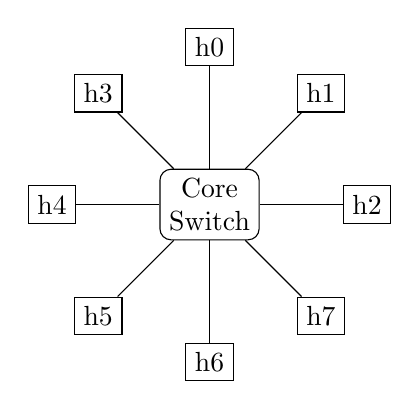
\begin{tikzpicture}
                        \node[draw,align=center,rounded corners] (s) at (0,0){Core\\Switch};
                        \node[draw] (h0) at (0,2){h0};
                        \node[draw] (h1) at ({sqrt(2)},{sqrt(2)}){h1};
                        \node[draw] (h2) at (2,0){h2};
                        \node[draw] (h3) at (-{sqrt(2)},{sqrt(2)}){h3};
                        \node[draw] (h4) at (-2,0){h4};
                        \node[draw] (h5) at (-{sqrt(2)},-{sqrt(2)}){h5};
                        \node[draw] (h6) at (0,-2){h6};
                        \node[draw] (h7) at ({sqrt(2)},-{sqrt(2)}){h7};
                    
                        \draw (h0) -- (s);
                        \draw (h1) -- (s);
                        \draw (h2) -- (s);
                        \draw (h3) -- (s);
                        \draw (h4) -- (s);
                        \draw (h5) -- (s);
                        \draw (h6) -- (s);
                        \draw (h7) -- (s);
                    \end{tikzpicture}
                    \caption{A single segment network (Figure~1.3)}
                    \label{fig:1.3}   
                \end{figure}
            \end{flushright}
        \end{minipage}
    \end{center}

\section{DHCP Server}
    In this exercise, we use \textit{h1} as the DHCP server. Configure the DHCP server by opening the configuration file\footnote{\path{/etc/dhcp/dhcpd.conf}} with a text editor such as \lstinline{nano}. To do this, run the following command:
    
	\fcolorbox{blue}{red!10}{{h\textsubscript{1}}'s Console}
    \lstset{backgroundcolor=\color{red!10}}
    \begin{lstlisting}
	nano /etc/dhcp/dhcpd.conf
    \end{lstlisting}
    
    Replace it with the configuration shown in \hyperref[tab:8.3]{Table~8.3}. (\textit{Note: }to do this, in \lstinline{nano} text editor, hold \lstinline{Ctrl+K} until all lines are cleared. Then, copy the given configuration to this file and save it). Then, do the following:

    \begin{enumerate}
        \item Replace the MAC address of \textit{h5} in server configuration file (\hyperref[tab:8.3]{Table~8.3}) by your \textit{h5} MAC address and save to \textit{dhcpd.conf}.
        
         \textbf{Note: }to obtain MAC address of \textit{h5} run the following command:
        
    \fcolorbox{blue}{red!10}{{h\textsubscript{5}}'s Console}
    \lstset{backgroundcolor=\color{red!10}}
    \begin{lstlisting}[xleftmargin=0.05in]
    ifconfig
    \end{lstlisting}
                
    \item Set the IP of \textit{h1} to {128.238.66.100}:
        
    \fcolorbox{blue}{red!10}{{h\textsubscript{1}}'s Console}
    \lstset{backgroundcolor=\color{red!10}}
    \begin{lstlisting}[xleftmargin=0.05in]
     ifconfig eth1 128.238.66.100/24
   	\end{lstlisting}
     	
     	
   \item Start the DHCP server on \textit{h1} in the foreground and working in the debugging mode:
        
    \fcolorbox{blue}{red!10}{{h\textsubscript{1}}'s Console}
    \lstset{backgroundcolor=\color{red!10}}
    \begin{lstlisting}[xleftmargin=0.05in]
    dhcpd -d -f
    \end{lstlisting}

        
    \item Run \lstinline{wireshark} to capture the DHCP messages in the network segment.
            
    \fcolorbox{blue}{lime!30}{{h\textsubscript{1}}'s Wireshark}
    \lstset{backgroundcolor=\color{lime!30}}
    \begin{lstlisting}[xleftmargin=0.05in]
	run wireshark on eth1
    \end{lstlisting}
        
        \item Then do the following to enable DHCP for the Ethernet interface on \textit{h2}. 
        
    \fcolorbox{blue}{red!10}{{h\textsubscript{2}}'s Console}
	\lstset{backgroundcolor=\color{red!10}}
	\begin{lstlisting}[xleftmargin=0.05in]
	ifconfig eth1 0
    dhclient eth1
    \end{lstlisting}

	\textbf{Note: }Running \lstinline{ifconfig eth1 0} clear IP of \textit{eth1} on \lstinline{h2}.

    When \textit{h2} is successfully reconfigured, execute \lstinline{ifconfig -a} or \lstinline{ip a} to display its
   network interface configurations and execute \lstinline{netstat -rn} or \lstinline{ip r} to display its routing table.
        
   	\fcolorbox{blue}{red!10}{{h\textsubscript{2}}'s Console}
    \lstset{backgroundcolor=\color{red!10}}
    \begin{lstlisting}[xleftmargin=0.05in]
    ifconfig -a
    \end{lstlisting}
    or
    
   	\fcolorbox{blue}{red!10}{{h\textsubscript{2}}'s Console}
   	\lstset{backgroundcolor=\color{red!10}}
    \begin{lstlisting}[xleftmargin=0.05in]
    ip a
    \end{lstlisting}
    
    Then,
    
   	\fcolorbox{blue}{red!10}{{h\textsubscript{2}}'s Console}
    \lstset{backgroundcolor=\color{red!10}}
    \begin{lstlisting}[xleftmargin=0.05in]
    netstat -rn
    \end{lstlisting}
    or
    
   	\fcolorbox{blue}{red!10}{{h\textsubscript{2}}'s Console}
   	\lstset{backgroundcolor=\color{red!10}}
    \begin{lstlisting}[xleftmargin=0.05in]
    ip r
    \end{lstlisting}
    
        Save the outputs for the lab report.
        
        \item Then, repeat 5 for \textit{h3}.
        
        \item Repeat 5 for \textit{h4}.
        
        \item Repeat 5 for \textit{h5}.
    \end{enumerate}

    Terminate \lstinline{wireshark}. Print out the DHCP messages for the lab report. 

    Save the DHCP server output on \textit{h1} for the lab report.

    \newpage
 
	\lstset{backgroundcolor=\color{cyan!10}}
    \begin{lstlisting}[language={conf}, caption={A DHCP server configuration file (Table~8.3)\label{tab:8.3}}]
	default-lease-time 600;
	max-lease-time 7200;
	option subnet-mask 255.255.255.0;
	option broadcast-address 128.238.66.255;
	option routers 128.238.66.1;
	#option domain-name-servers 128.238.2.38, 128.238.3.21;
	#option domain-name "netlab.ut.ac.ir";
	
	subnet 128.238.66.0 netmask 255.255.255.0 {
	    range 128.238.66.111 128.238.66.112;
	}
	
	host h5 {
	    hardware ethernet xx:xx:xx:xx:xx:xx;    	#Change this with h5's MAC address
	    fixed-address 128.238.66.110;
	}
    \end{lstlisting}

    \begin{report}
    \item Compare the DHCP operation captured by \lstinline{wireshark} and that shown by the DHCP server output.
    Explain how DHCP works.
    
    \item Did \textit{h2} and \textit{h3} successfully obtain a set of new parameters?
    Compare the \lstinline{ifconfig} and \lstinline{netstat} output with the parameters carried in the corresponding DHCP messages.
    
    \item Answer the above question for \textit{h4}.
    Explain why \textit{h4} failed.
    
    \item Answer the above question for \textit{h5}.
    Explain why \textit{h5} succeeded.
    \end{report}

\part{NTP exercises}
   Before proceeding to the next exercise, \underline{reboot the hosts} and set the network topology as given in \hyperref[fig:1.3]{Figure~1.3} and set the hosts IP addresses from 128.238.66.100 to 128.238.66.107.
    \begin{center}
        \begin{minipage}{0.48\textwidth}
            \begin{flushleft}
                \begin{table}[H]
                    \caption{The IP addresses of the hosts (Table~1.2)}
                    \centering
                    \begin{tabular}{ c c c }
                        \hline \hline
                        Host & IP Address & Subnet Mask \\
                        \hline 
                        h0 & 128.238.66.100 & 255.255.255.0 \\
                        h1 & 128.238.66.101 & 255.255.255.0 \\
                        h2 & 128.238.66.102 & 255.255.255.0 \\
                        h3 & 128.238.66.103 & 255.255.255.0 \\
                        h4 & 128.238.66.104 & 255.255.255.0 \\
                        h5 & 128.238.66.105 & 255.255.255.0 \\
                        h6 & 128.238.66.106 & 255.255.255.0 \\
                        h7 & 128.238.66.107 & 255.255.255.0 \\
                        \hline \hline
                        \label{table:1}
                        \end{tabular}
                \end{table}
            \end{flushleft}
        \end{minipage}
    \end{center}

\section{** Local Date}
   Execute \lstinline{date} to display the system time of your host(for example, \textit{h0}). Display the manual page of \lstinline{date}, and study its options and usages. Try the following \lstinline{date} commands:

    
    \fcolorbox{blue}{red!10}{{h\textsubscript{0}}'s Console}
    \lstset{backgroundcolor=\color{red!10}}
    \begin{lstlisting}
    date
    # after  display the system time 
    man date
	# after display the manual page of date
	date --date='2 days ago'
	# after  display the date
	date --date='3 months 2 days'
	# after  display the date
	date --set='+3 minutes'
	# after  display the date
	date -r /etc/network/interfaces
    \end{lstlisting}
\textbf{Note:} The sentences after \# are descriptions and  not need to enter them in \textit{h0}'s Console.
 
    For the last command, any other file can be used instead of \lstinline{/etc/network/interfaces}\footnote{This file is chosen because it is available in every host.}. 
    
    \begin{report}
    \item Submit the \lstinline{date} outputs you saved.
    Explain the use of the commands.
    \end{report}

\section{Remote Date}
   While \lstinline{wireshark} is running, execute \lstinline[emph={h1,netlab}]{rdate -p h1.netlab} on the \textit{h0} to display the system time of the \textit{h1} machine.
   Repeat the above \lstinline{rdate} command, but use the \lstinline{-u} option.
          
    \fcolorbox{blue}{lime!30}{{h\textsubscript{0}}'s Wireshark}
    \lstset{backgroundcolor=\color{lime!30}}
    \begin{lstlisting}
    Run wireshark on eth1, Filter: ip.addr == 128.238.66.100 && ip.addr == 128.238.66.101
       
    \end{lstlisting}
    
    \fcolorbox{blue}{red!10}{{h\textsubscript{0}}'s Console}
    \lstset{backgroundcolor=\color{red!10}}
    \begin{lstlisting}
    rdate -p 128.238.66.101
    \end{lstlisting}
    
    Now, repeat the above \lstinline{rdate} command but use the \lstinline{-u} option:
    
    \fcolorbox{blue}{red!10}{{h\textsubscript{0}}'s Console}
    \lstset{backgroundcolor=\color{red!10}}
    \begin{lstlisting}
    rdate -p 128.238.66.101 -u
    \end{lstlisting}
    
    Save the \lstinline{wireshark} output for the lab report.

    \begin{report}
    \item What port numbers were used by the remote machine?
    What port numbers were used by the local host?
    
    \item How many bytes of data were returned by the remote time server, both in the UDP case and in the TCP case?
    
    \item What TCP header options were used?
    \end{report}

\section{** NTP Sync}
    In this exercise, we start the NTP server daemon on \textit{h0} and use NTP to
    synchronize all the other hosts to \textit{h0}. Initially, study the NTP configuration file\footnote{\path{/etc/ntp.conf}} in \textit{h0}. 

    \fcolorbox{blue}{red!10}{{h\textsubscript{0}}'s Console}
    \lstset{backgroundcolor=\color{red!10}}
    \begin{lstlisting}
    nano /etc/ntp.conf
    \end{lstlisting}
    
    Now, start the NTP server on \textit{h0} by running below command:
    
    \fcolorbox{blue}{red!10}{{h\textsubscript{0}}'s Console}
    \lstset{backgroundcolor=\color{red!10}}
    \begin{lstlisting}
    service ntp start
    \end{lstlisting}

    To determine the status of the NTP server, execute the following command:
    
    \fcolorbox{blue}{red!10}{{h\textsubscript{0}}'s Console}
    \lstset{backgroundcolor=\color{red!10}}
    \begin{lstlisting}
    service ntp status
    \end{lstlisting}
    
Run \lstinline{wireshark} to capture packets between the \textit{h1} host and the \textit{h0}.
    
    \fcolorbox{blue}{lime!30}{h\textsubscript{1}'s Wireshark}
    \lstset{backgroundcolor=\color{lime!30}}
    \begin{lstlisting}
    Run wireshark on eth1, Filter: ip.addr == 128.238.66.100 && ip.addr == 128.238.66.101
       
    \end{lstlisting}
    
   
   Execute \lstinline{ntpdate -d -v 128.238.66.100} to synchronize the \textit{h1} host with \textit{h0}.
    
    \fcolorbox{blue}{red!10}{{h\textsubscript{1}}'s Console}
    \lstset{backgroundcolor=\color{red!10}}
    \begin{lstlisting}
    ntpdate -d -v 128.238.66.100
    \end{lstlisting}
    
    Study the output of this command and save the \lstinline{ntpdate} and the \lstinline{wireshark} outputs for the lab report.
    
    \begin{report}
    \item Which port does the NTP server use?
    Justify your answer using the \lstinline{wireshark} output.
    \end{report}

\section{** NTP Server}
    Keep the NTP server running on \textit{h0}. Run  \lstinline{wireshark} in any other host (e.g \textit{h1}) to capture the NTP messages between \textit{h1} and \textit{h0}:
    
    \fcolorbox{blue}{lime!30}{{h\textsubscript{1}}'s Wireshark}
    \lstset{backgroundcolor=\color{lime!30}}
    \begin{lstlisting}
    Run wireshark on eth1, Filter: ip.addr == 128.238.66.100 && ip.addr == 128.238.66.101
       
    \end{lstlisting}
    

    Edit the \path{/etc/ntp.conf} in \textit{h1} using a text editor such as \lstinline{nano}:
    
    \fcolorbox{blue}{pink!10}{{h\textsubscript{1}}'s Console}
    \lstset{backgroundcolor=\color{pink!10}}
    \begin{lstlisting}
    nano /etc/ntp.conf
    \end{lstlisting}
    
     Add the following line to the end of the config file, and save it by pressing \lstinline{Ctrl+X}, \lstinline{Y} and enter respectively.
    
    \fcolorbox{blue}{pink!10}{{h\textsubscript{1}'s NTP config}}
    \lstset{backgroundcolor=\color{pink!10}}
    \begin{lstlisting}[language={conf}]
    server 128.238.66.100
    \end{lstlisting}
    
    Start the NTP client on \textit{h1}, by executing:
    
    \fcolorbox{blue}{pink!10}{{h\textsubscript{1}}'s Console}
    \lstset{backgroundcolor=\color{pink!10}}
    \begin{lstlisting}
	service ntp start
    \end{lstlisting}
    
    Wait for several minutes. Then terminate the \lstinline{wireshark} program. Analyze the captured NTP packets. Print one of the NTP packets for the lab report.

    Execute the following command in \textit{h1} to get NTP server list: 
    
    \fcolorbox{blue}{pink!10}{{h\textsubscript{1}}'s Console}
    \lstset{backgroundcolor=\color{pink!10}}
    \begin{lstlisting}
    ntpq -p
    \end{lstlisting}

    Finally, execute \lstinline{ntptrace} in \textit{h1} to show the client/server relation of NTP:
    
    \fcolorbox{blue}{pink!10}{{h\textsubscript{1}}'s Console}
    \lstset{backgroundcolor=\color{pink!10}}
    \begin{lstlisting}
    ntptrace
    \end{lstlisting}
    

    \begin{report}
    \item Submit the NTP packet captured. List the fields and their values.
    
    \item What was the rate at which NTP queries were sent by the client?
    
    \item Which stratum was your host in? Which stratum was the NTP server in?
    \end{report}

\part{NAT Exercises}
    For the exercises in this section, we use a network setting as shown in \hyperref[fig:8.7]{Figure~8.7}. The lower subnet is a private network where the hosts are assigned with the Class A addresses with the 10.0.0.0/8 prefix. The upper subnet represents the Internet. The hosts, i.e.\  \textit{h0} and \textit{h1} are assigned with public IP addresses. Router 1 is used as the stub router, which performs address or port translation for the private network.
    \begin{figure}[H]
        \centering
        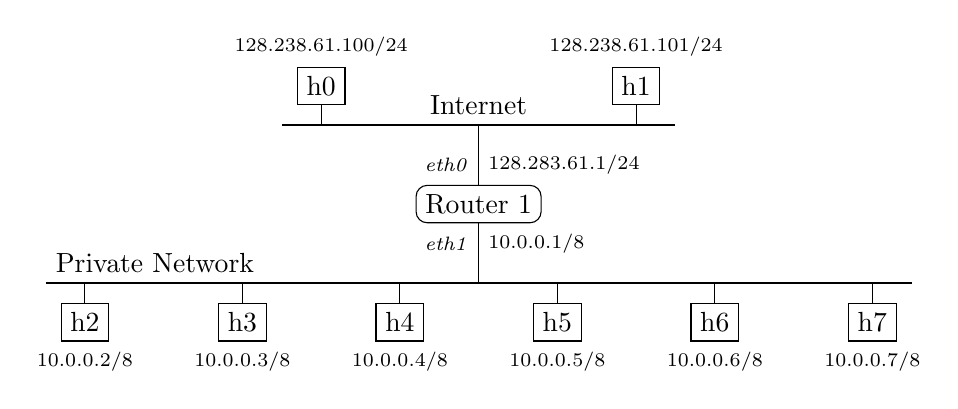
\begin{tikzpicture}
            \draw (0,0) node[draw,rounded corners,fill=white] (r1) {Router 1}
                -- +(0,1)
                -- +(0,-1)
                +(0,0.5) node[anchor=east] {\scriptsize\textit{eth0}}
                +(0,0.5) node[anchor=west] {\scriptsize128.283.61.1/24}
                +(0,-0.5) node[anchor=east] {\scriptsize\textit{eth1}}
                +(0,-0.5) node[anchor=west] {\scriptsize10.0.0.1/8}
            ;
            \draw (-1*2,1.5) node[draw,fill=white] (h0) {h0}
                -- +(0,-0.5)
                +(0,0.5) node {\scriptsize 128.238.61.100/24}
            ;
            \draw (1*2,1.5) node[draw,fill=white] (h1) {h1}
                -- +(0,-0.5)
                +(0,0.5) node {\scriptsize 128.238.61.101/24}
            ;
            \draw (-3*2+1,-1.5) node[draw,fill=white] (h2) {h2}
                -- +(0,0.5)
                +(0,-0.5) node {\scriptsize 10.0.0.2/8}
            ;
            \draw (-2*2+1,-1.5) node[draw,fill=white] (h3) {h3}
                -- +(0,0.5)
                +(0,-0.5) node {\scriptsize 10.0.0.3/8}
            ;
            \draw (-1*2+1,-1.5) node[draw,fill=white] (h4) {h4}
                -- +(0,0.5)
                +(0,-0.5) node {\scriptsize 10.0.0.4/8}
            ;
            \draw (1*2-1,-1.5) node[draw,fill=white] (h5) {h5}
                -- +(0,0.5)
                +(0,-0.5) node {\scriptsize 10.0.0.5/8}
            ;
            \draw (2*2-1,-1.5) node[draw,fill=white] (h6) {h6}
                -- +(0,0.5)
                +(0,-0.5) node {\scriptsize 10.0.0.6/8}
            ;
            \draw (3*2-1,-1.5) node[draw,fill=white] (h7) {h7}
                -- +(0,0.5)
                +(0,-0.5) node {\scriptsize 10.0.0.7/8}
            ;
            \draw[thick] (-2-0.5,1) -- +(2*2+1,0) node[pos=0.5,above] {Internet};
            \draw[thick] (-6+0.5,-1) -- +(6*2-1,0) node[pos=0,above,anchor=south west] {Private Network};
        \end{tikzpicture}
        \caption{The network configuration for the NAT exercises (Figure~8.7)}
        \label{fig:8.7}
    \end{figure}

\section{NAT}
	Connect the hosts and Router 1 as shown in \hyperref[fig:8.7]{Figure~8.7}. Then set the IP addresses and the network masks of your hosts as shown in the figure.
    Open R1's console and run the commands shown in \hyperref[tab:8.5]{Table~8.5} line by line. Note that there is a static translation that maps 10.0.0.7, or \textit{h7}, to 128.238.61.104.

    \newpage
    
    \fcolorbox{blue}{yellow!10}{{R\textsubscript{1}'s Console}}
    \lstset{backgroundcolor=\color{yellow!10}}
    \begin{lstlisting}[language={cisco}, emph={mypool}, caption={NAT Router Configuration in \hyperref[fig:8.7]{Figure~8.7} (Table~8.5)\label{tab:8.5}}]
    R1# conf term
	R1(config)# ip nat pool mypool 128.238.61.102 128.238.61.103 netmask 255.255.255.0
	R1(config)# ip nat inside source list 8 pool mypool
	R1(config)# ip nat inside source static 10.0.0.7 128.238.61.104
	R1(config)# int f0/0
	R1(config-if)# ip address 128.238.61.1 255.255.255.0
	R1(config-if)# no shut
	R1(config-if)# ip nat outside
	R1(config-if)# exit
	R1(config)# int f1/0
	R1(config-if)# ip address 10.0.0.1 255.0.0.0
	R1(config-if)# no shut
	R1(config-if)# ip nat inside
	R1(config-if)# exit
	R1(config)# access-list 8 deny host 10.0.0.7
	R1(config)# access-list 8 permit 10.0.0.0 0.0.0.255
	R1(config)# exit
    \end{lstlisting}
	
	Afterward, execute the following command to display the current router configuration:
	
	\fcolorbox{blue}{yellow!10}{{R\textsubscript{1}}'s Console}
	\lstset{backgroundcolor=\color{yellow!10}}
	\begin{lstlisting}[language={cisco}]
	R1# write term
	\end{lstlisting}

Execute \lstinline{show ip nat translations} in the router login window to display the translation table.
Save the output for the lab report.
	
	\fcolorbox{blue}{yellow!10}{{R\textsubscript{1}}'s Console}
	\lstset{backgroundcolor=\color{yellow!10}}
	\begin{lstlisting}[language={cisco}]
	R1# show ip nat translations
	\end{lstlisting}
	
	Save both outputs for the lab report.
	\begin{report}
	\item How many entries were there in the translation table? Why?
	\end{report}

\section{NAT Visibility}
    Keep the login session to the router running. Run \lstinline{wireshark} on two sides of the router (for example, \textit{h1} and  \textit{h5}).

    \fcolorbox{blue}{lime!30}{{h\textsubscript{1}}'s and {h\textsubscript{5}}'s Wireshark}
    \lstset{backgroundcolor=\color{lime!30}}
    \begin{lstlisting}
    Run wireshark on eth1
       
    \end{lstlisting}
    

    Before any host in the private network sends any packet out, \lstinline{ping} an inside host (e.g.\ \textit{h5}) from an outside host (e.g.\ \textit{h1}). You may try to \lstinline{ping} the following IPs. Can you \lstinline{ping} these IP addresses from \textit{h1}?
    
   \fcolorbox{blue}{red!10}{{h\textsubscript{1}'s Console}}
    \lstset{backgroundcolor=\color{red!10}}
    \begin{lstlisting}
    ping 128.238.61.102
    ping 128.238.61.103
    ping 128.238.61.104
    ping 10.0.0.5
    \end{lstlisting}
   

    Let an inside host send packets to an outside host, e.g.\ from \textit{h5}, execute:

    \fcolorbox{blue}{red!10}{{h\textsubscript{5}}'s Console}
    \lstset{backgroundcolor=\color{red!10}}
    \begin{lstlisting}
    ping 128.238.61.100
    \end{lstlisting}
    Can you \lstinline{ping} \textit{h5} from an outside host now? Why? Which IP address should be used in the \lstinline{ping} command in order to \lstinline{ping} \textit{h5}? (for example, run the below command):

   	\fcolorbox{blue}{red!10}{{h\textsubscript{1}'s Console}}
\lstset{backgroundcolor=\color{red!10}}
\begin{lstlisting}
    ping 128.238.61.102
\end{lstlisting}
    Execute the following command in the router console window to display the translation table. Save the output for the lab report: 
    
   	\fcolorbox{blue}{yellow!10}{{R\textsubscript{1}'s Console}}
    \lstset{backgroundcolor=\color{yellow!10}}
    \begin{lstlisting}[language={cisco}, frame=trBL]
    R1# show ip nat translations
    \end{lstlisting}
    
    \begin{report}
    \item Answer the above questions.
    Use the saved translation table to justify your answers.
    
    \item Compare the IP header of the ICMP query captured in the private network with that of the same ICMP query captured in the upper subnet, list their differences.
    Explain how NAT works.
    
    \item In addition to the IP address, what else was changed in the ICMP query packet?
    \end{report}

\section{** NAT Table}
    Keep the login session to the router running. Run \lstinline{wireshark} to capture ICMP messages on two subnet:
	
	\fcolorbox{blue}{lime!30}{{h\textsubscript{1}} and {h\textsubscript{2}}'s Wireshark}
    \lstset{backgroundcolor=\color{lime!30}}
    \begin{lstlisting}
    Run wireshark on eth1, Filter: icmp
       
    \end{lstlisting}
	
    Execute the following command on \textit{h2} to generate an ICMP port unreachable error:
    
    \fcolorbox{blue}{red!10}{{h\textsubscript{2}}'s Console}
    \lstset{backgroundcolor=\color{red!10}}
    \begin{lstlisting}
    socket -i -u -n1 128.238.61.101 8888
    \end{lstlisting}

    Print the ICMP error message for the lab report. 

    Execute the following command in the router console window to display the translation table and save the output for the lab report
    
    \fcolorbox{blue}{yellow!10}{{R\textsubscript{1}'s Console}}
    \lstset{backgroundcolor=\color{yellow!10}}
    \begin{lstlisting}[language=cisco, frame=trBL]
    R1# show ip nat translations
    \end{lstlisting}

    \begin{report}
    \item Analyze the IP headers, the ICMP headers, and the ICMP payloads of the ICMP port unreachable errors captured in the private network and in the public network from the first experiment.
    Explain how ICMP error was handled by the NAT router.
    \end{report}

\section{** NAT and PAT}
    Reboot the router to restore its default configuration(In GNS3, \textit{stop} the router and then \textit{start} it again). Then, configure the router to use PAT, as given in \hyperref[tab:8.6]{Table~8.6}. 

    \fcolorbox{blue}{yellow!10}{{R\textsubscript{1}'s Console}}
    \lstset{backgroundcolor=\color{yellow!10}}
    \begin{lstlisting}[language={cisco}, caption={PAT Router Configuration in \hyperref[fig:8.7]{Figure~8.7} (Table~8.6)\label{tab:8.6}}]
    	R1# conf term
    	R1(config)# ip nat inside source list 8 interface f0/0 overload
    	R1(config)# ip nat inside source static tcp 10.0.0.7 80 128.238.61.1 80
    	R1(config)# int f0/0
    	R1(config-if)# ip address 128.238.61.1 255.255.255.0
    	R1(config-if)# no shut
    	R1(config-if)# ip nat outside
    	R1(config-if)# exit
    	R1(config)# int f1/0
    	R1(config-if)# ip address 10.0.0.1 255.0.0.0
    	R1(config-if)# no shut
    	R1(config-if)# ip nat inside
    	R1(config-if)# exit
    	R1(config)# access-list 8 deny host 10.0.0.7
    	R1(config)# access-list 8 permit 10.0.0.0 0.0.0.255
    \end{lstlisting}
           
    Now all the hosts in the private network use the same IP address 128.238.61.1. However, note that there is a static translation that maps \textit{h7}’s port 80 to 128.238.61.1 port 80.

    Execute \lstinline{tcpdump} or \lstinline{wireshark} on both subnets, same as before.

    Generate traffic between the inside and outside hosts.
    Examine the \lstinline{tcpdump} or \lstinline{wireshark} output to see how PAT works.
    
    Start the Apache web server on \textit{h7}. 
    
    \fcolorbox{blue}{red!10}{{h\textsubscript{7}}'s Console}
    \lstset{backgroundcolor=\color{red!10}}
    \begin{lstlisting}[language=bash-ext]
    service apache2 start
    \end{lstlisting}
    
     Also, run the following command on an outside host (e.g.\ \textit{h0}).
    
    \fcolorbox{blue}{red!10}{{h\textsubscript{0}}'s Console}
    \lstset{backgroundcolor=\color{red!10}}
    \begin{lstlisting}[language=bash-ext]
    curl http://128.238.61.1
    \end{lstlisting}

    Execute the following command in the router's console window to display and then save the translation table:
	
	\fcolorbox{blue}{yellow!10}{{R\textsubscript{1}'s Console}}
	\lstset{backgroundcolor=\color{yellow!10}}
	\begin{lstlisting}[language=cisco, frame=trBL]
	R1# show ip nat translations
	\end{lstlisting}
	
    \begin{report}
    \item From the \lstinline{wireshark} data, explain how PAT worked, both for a dynamic translation and a static translation.
    
    \item With PAT, can you have two web servers in the private network?
    If not, why?
    If yes, explain how this can be done.
    \end{report}

\part{** Socket Programming Exercises}
\section{Socket Programming}

	For the exercises in this section, use a simple network topology with two terminal hosts, as shown in \hyperref[fig:two-term]{Figure~6}.
 	\begin{figure}[H]
		\centering
		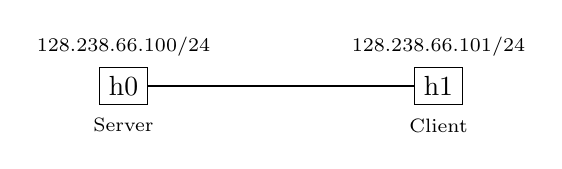
\begin{tikzpicture}
		\node[draw] (h1) at (2,0){h1};
		\node[draw] (h0) at (-2,0){h0};
		
		\draw (h0) -- (h1);
		\draw (h1) +(0,0.5) node {\scriptsize 128.238.66.101/24};
		\draw (h1) +(0,-0.5) node {\scriptsize Client};
		\draw (h0) +(0,0.5) node {\scriptsize 128.238.66.100/24};
		\draw (h0) +(0,-0.5) node {\scriptsize Server};
		\end{tikzpicture}
		\caption{Two simple hosts connected directly.}
		\label{fig:two-term}
	\end{figure}
	
    Examine the UDP socket programs \path{/home/netlab/code/UDPserver.c} and \path{/home/netlab/code/UDPclient.c} to learn how to write a UDP socket program. First, navigate to the codes directory:
    
    \fcolorbox{blue}{pink!10}{{h\textsubscript{0}}'s Console}
    \lstset{backgroundcolor=\color{pink!10}}
    \begin{lstlisting}
    cd /home/netlab/code
    \end{lstlisting}
    
    \fcolorbox{blue}{pink!10}{{h\textsubscript{1}}'s Console}
    \lstset{backgroundcolor=\color{pink!10}}
    \begin{lstlisting}
    cd /home/netlab/code
    \end{lstlisting}
    
    Now open the files with a text editor:
    
    \fcolorbox{blue}{pink!10}{{h\textsubscript{0}}'s Console}
    \lstset{backgroundcolor=\color{pink!10}}
    \begin{lstlisting}
    nano UDPserver.c
    \end{lstlisting}
    
    \fcolorbox{blue}{pink!10}{{h\textsubscript{1}}'s Console}
    \lstset{backgroundcolor=\color{pink!10}}
    \begin{lstlisting}
    nano UDPclient.c
    \end{lstlisting}
    
    You can compile the C programs by using the following commands. Compile output available is at \path{/usr/local/bin/} directory:

    \fcolorbox{blue}{pink!10}{{h\textsubscript{0}}'s Console}
	\lstset{backgroundcolor=\color{pink!10}}
	\begin{lstlisting}
	gcc -o UDPserver UDPserver.c -lnsl
	\end{lstlisting}
	
    \fcolorbox{blue}{pink!10}{{h\textsubscript{1}}'s Console}
	\lstset{backgroundcolor=\color{pink!10}}
	\begin{lstlisting}
	gcc -o UDPclient UDPclient.c -lnsl
	\end{lstlisting}
	
    Start \lstinline{wireshark} to capture packets between these two hosts.
    
    On the \textit{h0}, start the UDP server by executing: (server-port can be any port unused by the system)
    
    \fcolorbox{blue}{pink!10}{{h\textsubscript{0}}'s Console}
   	\lstset{backgroundcolor=\color{pink!10}}
   	\begin{lstlisting}[emph={server-port}]
   	./UDPserver server-port
   	\end{lstlisting}
    
    Then, start the UDP client on \textit{h1} by running:
    
    \fcolorbox{blue}{pink!10}{{h\textsubscript{1}}'s Console}
   	\lstset{backgroundcolor=\color{pink!10}}
   	\begin{lstlisting}[emph={server-port, a-message}]
   	./UDPclient 128.238.66.100 server-port a-message
   	\end{lstlisting}
   
    Where the \lstinline{server-port} is same as before and \lstinline{a-message} is any string. You may execute the UDP client program on other hosts to connect to the same UDP server.

    Terminate \lstinline{wireshark}, examine its output and compare the output with the UDP server and client outputs.

    Repeat the above experiments, but now use the \lstinline{TCPserver.c} and \lstinline{TCPclient.c} instead of \lstinline{UDPserver.c} and \lstinline{UDPclient.c}.

\section{Socket Options}
    
    Study the applications of \lstinline{setsockopt} function in socket programming by reading the documents or manual pages available in internet.
    %Execute the following command to display the various socket options and how to set them:

	%\fcolorbox{blue}{yellow!10}{{h\textsubscript{0}}}
	%\lstset{backgroundcolor=\color{yellow!10}}
	%\begin{lstlisting}[emph={server-port, a-message}]
	%man setsockopt
	%\end{lstlisting}

    Examine the \lstinline{netspy} and \lstinline{netspyd} source code in Appendix~C.2 of reference book to see how to create a multicast socket and how to set the TTL value for the packets.
    
    % \begin{report}
    % \item Explain the various options you could set on socket.
    % \item Explain the difference between a socket and multicast socket.
    % \end{report}

\section{FTP Socket Programming}
    This is an optional exercise on socket programming. Or, it can be assigned as a take-home project for extra credits. Note that familiarity with C (or C++) programming is required.

    \subsection*{Problem}
    Examine the message exchanges of FTP. Write a FTP client program which takes a file name as input, and upload the file to a standard FTP server on a remote machine.

    \subsection*{Hints}
    \begin{itemize}
        \item First you need to set up the control connection to Port 21 of the remote machine, using a TCP socket.
        \item When the control connection is established, you need to exchange FTP commands with the remote FTP server, as given in \hyperref[tab:5.1]{Table~5.1} of reference book.
        \item You can first run the following commands to list all the FTP commands:
        
	\fcolorbox{blue}{pink!10}{{h\textsubscript{1}}'s Console}
    \lstset{backgroundcolor=\color{pink!10}}
        \begin{lstlisting}[xleftmargin=0.05in]
    telnet 128.238.66.100 21
    help
    \end{lstlisting}
        
    Also, you can try the commands out in the \lstinline{telnet} window, e.g.\ use the following commands to send the user ID and the password to the FTP server:
        
    \fcolorbox{blue}{pink!10}{{h\textsubscript{1}'s telnet}}
    \lstset{backgroundcolor=\color{pink!10}}
        \begin{lstlisting}[xleftmargin=0.05in]
    USER netlab
    PASS netlab
    \end{lstlisting}
        
        To terminate the \lstinline{telnet} session, type \lstinline{QUIT}.
        \item In your program, these messages should be sent to the FTP server by calling the \lstinline{send()} function of the local TCP socket.
        \item Also your program needs to parse the server responses (some examples are given in \hyperref[tab:5.2]{Table~5.2} of reference book) to find out the status of the previous FTP command.
        \item The FTP data connection should be established using the \lstinline{PORT} command (see Chapter~5 of reference book).
    \end{itemize}

\end{document}